\documentclass[../Interim_Report_Master]{subfiles}
\begin{document}
\hypertarget{drop_mod}{\section{Droplet Evaporation Model}\label{drop_mod}}
\subsection{Definition of Models} 
The 8 models in \cite{Miller1998} are denoted by Mx where x is the model number.

What defines the models are the variables \(f_{1}\), \(f_{2}\), \(Nu\), \(Sh\) \(H_{\Delta T}\) and \(H_{M}\). Although the main variation in the models stems from \(f_{2}\), \(H_{\Delta T}\) and \(H_{M}\). M1 is known as the classical rapid mixing model. M2 will be ruled out for the purposes of this project as the $B'_T$ term in the evaporation correction $f_2$ must be solved iteratively at each timestep. This increases the computation overhead of the simulation which may be acceptable for a single droplet but will be problematic for large population of droplets.
\begin{table}[h]
	\centering
	\begin{tabular*}{\textwidth}{c @{\extracolsep{\fill}} cccc}
		\hline
		\textbf{Model} & \textbf{Name} & \textbf{$f_2$} & \textbf{$H_{\Delta T}$} & \textbf{$H_M$} \\ \hline
		\textbf{M1} & Classical rapid mixing & $1$ & $0$ & $\ln \left[1+B_{M,eq}\right]$ \\[2ex] 
		\textbf{M2} & Abrmazon-Sirignano & $\frac{-\dot{m}_{d}}{{m}_{d}B'_{T}}\left[\frac{3Pr_{G}\tau_{d}}{Nu}\right]$ & $0$ & $\ln \left[1+B_{M,eq}\right]$ \\[2ex] 
		\textbf{M3} & Mass analogy Ia & $1$ & 0 & $B_{m,eq}$ \\[2ex]
		\textbf{M7} & Langmuir-Knudsen I & $\frac{\beta}{e^{\beta}-1}$ & $\frac{2\beta}{3Pr_G}\left(\frac{\theta_1}{\tau_d}\right)\Delta_s$ & $\ln \left[1+B_{M,neq}\right]$ \\[2ex] \hline
	\end{tabular*}
	\caption{Detail of variables used in candidate models.}
\end{table}

A more suitable model to provide a point of comparison in this case would be one of the mass analogy models, M3-M6. Which are derived from vapour mass fraction boundary condition at the droplet's surface. This assumes the droplet does not dissolve in the gas phase. These models use the same formulations for the surface vapour mass fraction ($Y_s$), Spalding transfer number for mass ($B_m$) and mass transfer potential ($H_{\Delta T}$). This would simplify producing code for an extra model.

Models M7 and M8, are to be ruled out as they use non-equilibrium formulations of the coefficients which would further complicate the code. The comparison between models is left as future work. With the choice of model for this project will be M1 due to its wide usage and ease of implementation.

\subsection{Assumptions}
The model presented here is subject to the following assumptions:
\begin{enumerate}
	\item The droplets are formed of a single species
	\item The droplet is spherical and remains spherical for the entire evaporation process
	\item There is no interaction between droplets
	\item Within the droplet there is 
		\begin{enumerate}
			\item Zero temperature gradient
			\item Zero concentration gradient
		\end{enumerate}
	\item The droplet temperature is homogeneous
	\item The properties of the carrier gas are constant and are unaffected by the process of droplets evaporating
\end{enumerate}

\cite{Miller1998}\cite{arnold2000}.

\subsection{Governing Equations}
Each of the models are defined by the same four Lagrangian equations for the droplets:
\begin{align}
\frac{dX_{i}}{dt} &= v_{i} 
\label{vel} \\
\frac{dv_{i}}{dt} &= \left(\frac{f_{1}}{\tau_{d}}\right)(u_{i}-v_{i}) + g_i 
\label{accel} \\
\frac{dT_{d}}{dt} &= \frac{f_{2}Nu}{3Pr_{G}}\left(\frac{\theta_1}{\tau_d}\right)(T_{G}-T_{d}) + \left(\frac{L_{V}}{C_{L}}\right)\frac{\dot{m}_{d}}{m_{d}} - H_{\Delta T} 
\label{temp} \\
\frac{dm_{d}}{dt} &= -\frac{Sh}{3Sc_{G}}\left(\frac{m_{d}}{\tau_{d}}\right)H_M
\label{mass}
\end{align}

\subsubsection{Particle Timescales}
$\tau_d$ is the momentum relaxation timescale for the particle. Which is the time it takes for the droplet to adjust to changes in the gas flow \cite{holterman2012}. This provides a timescale for each particle. It is determined from:
\begin{equation}
\tau_d = \frac{\rho_d D^2}{18\mu_G}
\end{equation}

There is an equivalent timescale for the heat transfer process. This can be derived from equation \ref{heat_sol_an} as:
\begin{equation}
\tau_h = \tau_d\left(\frac{3Pr_G}{Nu f_2 \theta_1}\right)
\end{equation}

These two timescales are exceptionally useful for the non-dimensionalisation of results. This provides a way of evaluating how quickly processes occur in the timescale of the particle. Which is a far more useful insight into the physics taking place than particle x takes y seconds to evaporate.

\subsubsection{Position}
Equation \ref{vel} and a simpler form of equation \ref{accel} were used in the IP this project is based off. The differential equation for position was solved using the trapezoidal rule, as this method has second order accuracy and the result is a linear first order equation \cite{Elijah_GPU_Report}. 
\begin{equation}
X_{n+1} = X_{n} + \frac{v_{n}+v_{n+1}}{2} \Delta t
\end{equation}

\subsubsection{Velocity}\label{sec:vel}
For equation \ref{accel}, the acceleration of the droplet is defined using Stokes' Law and can be derived by considering the forces acting on the particle:
\begin{figure}
	\centering
	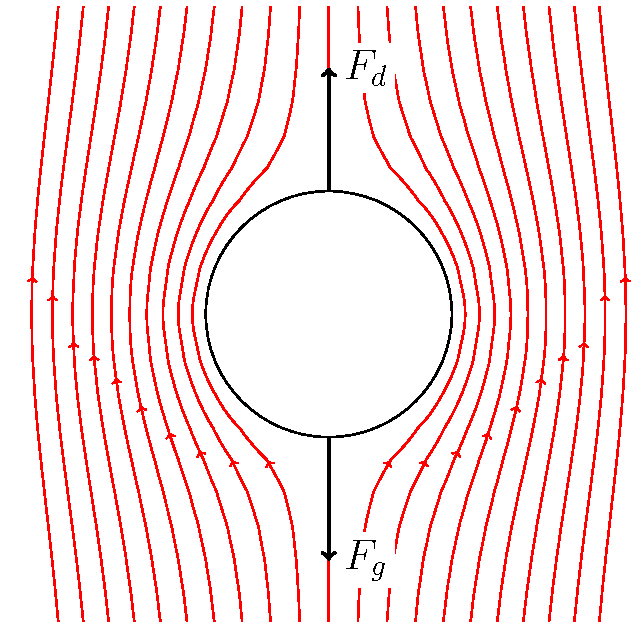
\includegraphics[width=0.5\textwidth, trim=12 0 6 0, clip]{./Diagrams/Particle_Forces/Particle_Forces.pdf}
	\caption{Forces acting on a particle under a Stokes flow regime.}
	\label{particle_forces}
\end{figure}

The total force acting on the particle is:
\begin{equation}
F = F_g + F_d
\end{equation}

This can be solved as a differential equation:
\begin{subequations}
	\begin{align}
	F &= ma \\
	F &= m\frac{du}{dt} \\
	\frac{du}{dt} &= \frac{F(u)}{m}
	\end{align}
\end{subequations}

The force acting on the particle is the sum of the weight and drag forces. The weight force is given by:
\begin{equation}
F_g = mg
\end{equation}

It is assumed the particle experiences a Stokes drag regime, therefore:
\begin{equation}
F_d = \frac{m}{\tau_d}(u_f-u)
\end{equation}

So, the differential equation is:
\begin{subequations}
	\begin{align}
	\frac{du}{dt} &= \frac{F(u)}{m} \\
	\frac{du}{dt} &= \frac{F_g + F_d}{m} \\
	\frac{du}{dt} &= \frac{mg + \frac{m}{\tau_d}(u-v)}{m} \\
	\frac{du}{dt} &= \frac{1}{\tau_d}(u-v) + g
	\end{align}
\end{subequations}

This is for one vector component, hence the general case is:
\begin{equation}
\frac{dv_i}{dt} = \frac{1}{\tau_d}(u_i-v_i) + g_i
\end{equation}

This change in velocity is dependent on three terms. Acceleration due to gravity \(g_{i}\), and the difference between the carrier gas velocity and the velocity of the particle, \(u_{i}-v_{i}\). The third term is a correction for Stokes drag that is dependent on the time constant for Stokes flow. 

A formulation for $f_1$ is given in \cite{Miller1998} as:
\begin{equation}
f_{1} = \frac{1+0.0545Re_{d}+0.1Re_{d}^{0.5}(1-0.03Re_{d})}{1+a|Re_{b}|^{b}}
\end{equation}

With the Reynolds numbers defined as:
\begin{subequations}
\begin{align}
Re_d &= \frac{\rho_G u_s D}{\mu_G} \\
Re_b &= \frac{\rho_G u_b D}{\mu_G} 
\intertext{The velocities defined as:}
u_s &= |u_i-v_i| \\
u_b &= -\frac{\dot{m}}{\pi \rho_G D^2 u_b}
\intertext{And the constants $a$ and $b$ defined as:}
a &= 0.09 + 0.077\exp(-0.4Re_d) \\
b &= 0.4 + 0.77\exp(-0.04Re_d)
\end{align}
\end{subequations}

Which is an empirical result produced from a data fit. In this format it is valid for $0\leq Re_d \leq 100$ and $0\leq Re_b \leq 10$. For the purpose of this research $f_1$ will be set to $1$. This reduces the computation per timestep and still allows for comparisons to be made with data in the literature. As the models can be driven by iterating from an initial Reynolds number instead of using equation \ref{accel}.

\subsubsection{Temperature}
The temperature ODE can be derived using the general energy conservation equation and application of non-dimensional numbers. 

From the energy conservation equation and using the using the definition for the change in enthalpy:
\begin{subequations}
\begin{align}
\dot{Q} - \dot{E} &= \frac{dH_d}{dt} \\
Q_L &= \frac{dH_d}{dt}
\end{align}
\end{subequations} 

Using the definition for specific enthalpy $h_d(dm_d/dt) + m_d(dh_d/dt)$ and the approximation $dh_d=C_{p,d} dT_d$ leads to the temperature ODE \cite{protheroe2014}.
\begin{equation}
\frac{dT_{d}}{dt} = \frac{f_{2}Nu}{3Pr_{G}}\left(\frac{\theta_1}{\tau_d}\right)(T_{G}-T_{d}) + \left(\frac{L_{V}}{C_{L}}\right)\frac{\dot{m}_{d}}{m_{d}} - H_{\Delta T} 
\end{equation}

The term $H_{\Delta T}$ is a correction factor to include effects from a non-uniform internal temperature \cite{Miller1998}.

\subsubsection{Mass}\label{sec:mass_mod}
Using the conservation equations from Section \ref{sec:mass_transfer} the mass transfer ODE can be derived.

First, the continuity equation can be simplified as the model assumes quasi-steady conditions:
\begin{subequations}
\begin{align}
\frac{\partial(\rho u r^2)}{\partial r} &= \rho u r^2 = constant \\
\rho u r^2 &= \frac{\dot{m}}{4\pi}
\end{align}
\end{subequations}

The equation from the vapour phase equilibrium can also be simplified using the quasi-steady assumption:
\begin{subequations}
\begin{align}
\frac{\partial}{\partial r}(\rho_G r^2 u Y ) - \frac{\partial}{\partial r}(\rho_G r^2 \Gamma_G \frac{\partial Y}{\partial r}) &= 0 \\
(\rho_G r^2 u Y ) - (\rho_G r^2 \Gamma_G \frac{dY}{dr}) &= 0
\end{align}
\end{subequations}

Combining this with the continuity equation:
\begin{subequations}
\begin{align}
(\rho_G r^2 u Y ) - (\rho_G r^2 \Gamma_G \frac{dY}{dr}) &= \frac{\dot{m}}{4\pi} \\
(4 \rho_G r^2 \Gamma_G \frac{dY}{dr}) &= \dot{m}(Y-1)
\end{align}
\end{subequations}

Integration and application of the droplet surface boundary condition obtains an equation for vaporisation rate:
\begin{equation}
\dot{m} = 4\pi \rho_G \Gamma_G r_d \ln(1+B_M)
\end{equation}

Application of relations for the Sherwood and Schmidt numbers gives the final mass ODE \cite{sirignano_1999}.
\begin{equation}
\frac{dm_d}{dt} = -\frac{Sh}{3Sc_G}\frac{m_d}{\tau_d}H_M
\end{equation}

\subsubsection{Reference Properties}
The well known ``1/3 rule'' is often used for evaluating a reference temperature $T_R$ and a reference mass fraction $Y_R$ \cite{Miller1998} \cite{Shashank2011} \cite{SacomanoFilho2019} \cite{Kolaitis2006} \cite{Aggarwal1984}. The reference mass fraction is then used in mixture calculations, for example the Wilke rule to evaluate the diffusive properties. \cite{Miller1998} shows these mixture calculations are not necessary for common experimental test cases in the literature. So, mixture calculations will not be used here. 

The reference temperature is used for determining gas and vapour properties. For this instead of the ``1/3 rule'' an estimated value for the wet bulb temperature $T_{WB}$ of the droplet is used. If the bulb of a thermometer is covered with a damp cloth the temperature that is read from it is the wet bulb temperature. This is lower than the dry bulb temperature as heat energy transferred from the gas is used to evaporate moisture in the cloth. In the context of droplet evaporation the wet bulb temperature can be considered the temperature at the surface of the droplet \cite{lukashov2003}. And this value can be used for the gas and vapour phase property evaluation. \cite{Miller1998} provides a correlation fit for $T_{WB}$ as:
\begin{equation}
T_{WB} = 137\left(\frac{T_B}{373.115}\right)^{0.68}\log_{10}(T_G) - 45
\end{equation}

This will be used as the reference temperature.

\subsection{Model Evaluation}
\subsubsection{Property Evaluation}
Following the method used in \cite{Miller1998} the gas and vapour properties will be evaluated once at the start of the simulation using the reference conditions.

The process for getting the properties is as follows:
\begin{enumerate}
	\item Set droplet physical properties:
		\begin{enumerate}
			\item $W_V$
			\item $T_B$
			\item $\rho_d$
			\item $C_L$
		\end{enumerate}
	\item Set fluid physical properties:
		\begin{enumerate}
			\item $W_G$
			\item $\theta_2$ from $W_V$ and $W_G$
			\item $P_{atm}$
			\item $R_{bar}$
			\item $R$
			\item $Y_G$
		\end{enumerate}
	\item Get reference conditions:
		\begin{enumerate}
			\item $T_{WB}$ using $T_B$ and $T_G$. $T_{WB}$ is used as $T_R$
		\end{enumerate}
	\item Set additional droplet physical properties:
		\begin{enumerate}
			\item $L_V$ using $T_R$
		\end{enumerate}
	\item Set additional fluid physical properties:
		\begin{enumerate}
			\item $P_G$ using the ideal gas law with $T_R$ and $\rho_G$
			\item $\mu_G$ using $T_R$
			\item $Pr_G$ using $T_R$
			\item $Sc_G$ equal to $Pr_G$ (assuming unity Lewis (Le) number)
		\end{enumerate}
	\item Set additional properties:
		\begin{enumerate}
			\item $H_{\Delta T}$ 
			\item $f_2$
			\item $\theta_1$ using $C_{p,G}$ and $C_L$
		\end{enumerate}	
\end{enumerate}

The droplet and fluid physical properties used can be found in Section x. $\rho_G$ and $C_{p,G}$ are also obtained from reference data that can be found in Section \ref{sec:phys_data}. Running the model also requires inputting the following:
\begin{enumerate}
	\item $D_0$
	\item $T_{d0}$
	\item $T_G$
	\item $u_i$ or $Re_{d0}$
\end{enumerate}

In the case of using $Re_{d0}$ this value is used as $Re_d$ which remains fixed during the simulation.

It should be noted M1 normally uses the the ``1/3 rule'' at each timestep. The usage of the model is in contrast to the literature but it is shown in Section \ref{sec:heat_mass_val} the results are still within reason. 

\subsubsection{Evaluation of Properties During a Timestep}
For a single timestep the procedure is:
\begin{enumerate}
	\item Calculate the mass fractions:
		\begin{enumerate}
			\item $\chi_{s,eq}$
			\item $Y_{s,eq}$
			\item $B_{M,eq}$
			\item $H_M$
		\end{enumerate}
	\item Calculate non-dimensional numbers:
	\begin{enumerate}
		\item $Re_d$
		\item $Sh$
		\item $Nu$
	\end{enumerate}
	\item Get the rate of change of mass $\dot{m_d}$ 
	\item Get the change in temperature $dT_d/dt$
	\item Update the mass $m_d$
	\item Update the temperature $T_d$
\end{enumerate}

The process of getting the mass fractions can be further broken down. $H_M$ is calculated in the case of M1 using:
\begin{equation}
H_M=\ln\left[1+B_{M,eq}\right]
\end{equation}

Where $B_{M,eq}$ is the Spalding transfer number for mass transfer given by:
\begin{equation}
B_{M,eq} = \frac{Y_{s,eq}-Y_G}{1-Y_{s,eq}}
\end{equation}

With $Y_G$ the free stream vapour mass fraction and $Y_{s,eq}$ the vapour mass fraction at the droplet's surface:
\begin{equation}
Y_{s,eq} = \frac{\chi_{s,eq}}{\chi_{s,eq}+(1-\chi_{s,eq})\theta_2}
\end{equation}

$\chi_{s,eq}$ is the surface equilibrium mole fraction of the vapour and $\theta_2$ is the ratio of molecular weights:
\begin{equation}
\theta_2=\frac{W_C}{W_V}
\end{equation}

The Clausius-Clapeyron equation for constant latent heat gives a relation between the saturation pressure $P_{sat}$ and the free stream pressure $P_G$ as:
\begin{subequations}
	\begin{align}
	\chi_{s,eq} =& \frac{P_{sat}}{P_G} \\
	\chi_{s,eq} =& \frac{P_{atm}}{P_G}\exp \left[\frac{L_V}{\bar{R}/W_V}\left(\frac{1}{T_B}-\frac{1}{T_d}\right)\right] 
	\end{align}
\end{subequations}
\end{document}